\documentclass[10pt]{article}
\usepackage[utf8]{inputenc}
\usepackage[T1]{fontenc}
\usepackage{amsmath}
\usepackage{amsfonts}
\usepackage{amssymb}
\usepackage{mhchem}
\usepackage{stmaryrd}
\usepackage{graphicx}
\usepackage[export]{adjustbox}
\graphicspath{ {./} }

\begin{document}
Citation: Cohen, B., Lai, W. M., \& Mow, V. C. (1998). A transversely isotropic biphasic model for unconfined compression of growth plate and chondroepiphysis.

\section{Parameters}
Choose the following parameters and compute the inversion
$$
\begin{gathered}
E_{1}=8.5 \mathrm{kPa}, \quad E_{3}=19 \mathrm{kPa}, \quad v_{21}=0.75, \quad v_{31}=0.24 \\
t_{g}=40.62 \mathrm{sec}, \quad \dot{\varepsilon}_{0}=0.01 \mathrm{sec}^{-1} \\
t_{0} / t_{g}=0.25
\end{gathered}
$$

\section{Setup Equations}
$$
\begin{aligned}
&\Delta_{1}=1-v_{21}-2 v_{31}^{2} \frac{E_{1}}{E_{3}} \\
&\Delta_{2}=\left(1-v_{31}^{2} \frac{E_{1}}{E_{3}}\right) /\left(1+v_{21}\right) \\
&\Delta_{3}=\left(1-2 v_{31}^{2}\right) \frac{\Delta_{2}}{\Delta_{1}}
\end{aligned}
$$
$$
C_{11}=\frac{E_{1} \cdot\left(1-v_{31}^{2} \frac{E_{1}}{E_{3}}\right)}{\left(1+v_{21}\right) \cdot \Delta_{1}}
$$
$$
C_{12}=\frac{E_{1} \cdot\left(v_{21}+\frac{v_{31}^{2} E_{1}}{E_{3}}\right)}{\left(1+v_{21}\right) \cdot \Delta_{1}}
$$
$$
C_{13}=\frac{E_{1} v_{31}}{\Delta_{1}}=\frac{E_{1} v_{31}}{1-v_{21}-2 v_{31}^{2} \frac{E_{1}}{E_{3}}}
$$
$$
C_{33}=E_{3} \cdot\left(1+\frac{2 v_{31}^{2} \frac{E_{1}}{E_{3}}}{\Delta_{1}}\right)=\frac{E_{3}\left(\Delta_{1}+2 v_{31}^{2} \frac{E_{1}}{E_{3}}\right)}{\Delta_{1}}=\frac{\Delta_{1} E_{3}+2 v_{31}^{2} E_{1}}{\Delta_{1}}
$$
$$
\begin{aligned}
&C_{0}=\frac{C_{11}-C_{12}}{C_{11}} \\
&C_{1}=\frac{C_{11}+C_{12}-4 C_{13}+2 C_{33}}{C_{11}-C_{12}} \\
&C_{2}=2 \cdot \frac{C_{33}\left(C_{11}-C_{12}\right)+C_{11}\left(C_{11}+C_{12}-4 C_{13}\right)+2 C_{13}^{2}}{\left(C_{11}-C_{12}\right)^{2}}
\end{aligned}
$$
Units of $C_{11}, C_{12}, C_{13}$ are in $\mathrm{kPa}$ (the same dimension as $E_{1}$ and $E_{3}$ )

Units of $C_{0}, C_{1}, C_{12}$ are non-dimensional

Units of $\Delta_{0}, \Delta_{1}, \Delta_{2}$ are non-dimensional

\section{Laplace Solution}
$$
\tilde{\varepsilon}_{z z}=\dot{\varepsilon}_{0} \cdot t_{g} \cdot \frac{1-\exp \left(-s \cdot t_{0} / t_{g}\right)}{s^{2}}
$$
Finally:

$\widetilde{F(s)}=\tilde{\varepsilon}_{Z Z} \cdot \frac{C_{1} I_{0}[\sqrt{s}]-C_{2} \cdot C_{0} \cdot \frac{I_{1}[\sqrt{s}]}{\sqrt{s}}}{I_{0}[\sqrt{s}]-C_{0} \cdot \frac{I_{1}[\sqrt{s}]}{\sqrt{s}}}$

\section{Inversion (Time) Solution}
$$
\begin{aligned}
&f(t)=E_{3} \dot{\varepsilon}_{0} t+E_{1} \dot{\varepsilon}_{0} t_{g} \Delta_{3}\left(\frac{1}{8}-\sum \frac{\exp \left(-\frac{\alpha_{n}^{2} t}{t_{g}}\right)}{\alpha_{n}^{2}\left[\Delta_{2}^{2} \alpha_{n}^{2}-\frac{\Delta_{1}}{1+v_{21}}\right]}\right) \text { if } \mathrm{t}<t_{0} \\
&f(t)=E_{3} \dot{\varepsilon}_{0} t_{0}-E_{1} \dot{\varepsilon}_{0} t_{g} \Delta_{3}\left(\sum_{\alpha_{n}^{2}} \frac{\exp \left(-\frac{\alpha_{n}^{2} t}{t_{g}}\right)-\exp \left(-\frac{\alpha_{n}^{2}\left(t-t_{0}\right)}{t_{g}}\right)}{\alpha_{n}^{2}\left[\Delta_{2}^{2} \alpha_{n}^{2}-\frac{\Delta_{1}}{1+v_{21}}\right]}\right) \quad \text { if } \mathrm{t} \geq t_{0}
\end{aligned}
$$

\section{Limit in Time Case}
$$
\begin{gathered}
\lim _{t \rightarrow \infty} f(t)=E_{3} \dot{\varepsilon}_{0} t_{0}-E_{1} \dot{\varepsilon}_{0} t_{g} \Delta_{3} \lim _{t \rightarrow \infty}\left(\sum_{\alpha_{n}^{2}} \frac{\exp \left(-\frac{\alpha_{n}^{2} t}{t_{g}}\right)-\exp \left(-\frac{\alpha_{n}^{2}\left(t-t_{0}\right)}{t_{g}}\right)}{\alpha_{n}^{2}\left[\Delta_{2}^{2} \alpha_{n}^{2}-\frac{\Delta_{1}}{1+v_{21}}\right]}\right) \\
=E_{3} \dot{\varepsilon}_{0} t_{0}-E_{1} \dot{\varepsilon}_{0} t_{g} \Delta_{3} \lim _{t \rightarrow \infty}\left(\sum_{\alpha_{n}^{2}} \frac{0-0}{\alpha_{n}^{2}\left[\Delta_{2}^{2} \alpha_{n}^{2}-\frac{\Delta_{1}}{1+v_{21}}\right]}\right)=E_{3} \dot{\varepsilon}_{0} t_{0}
\end{gathered}
$$
Variable Manipulation to Help Laplace Limit Derivation

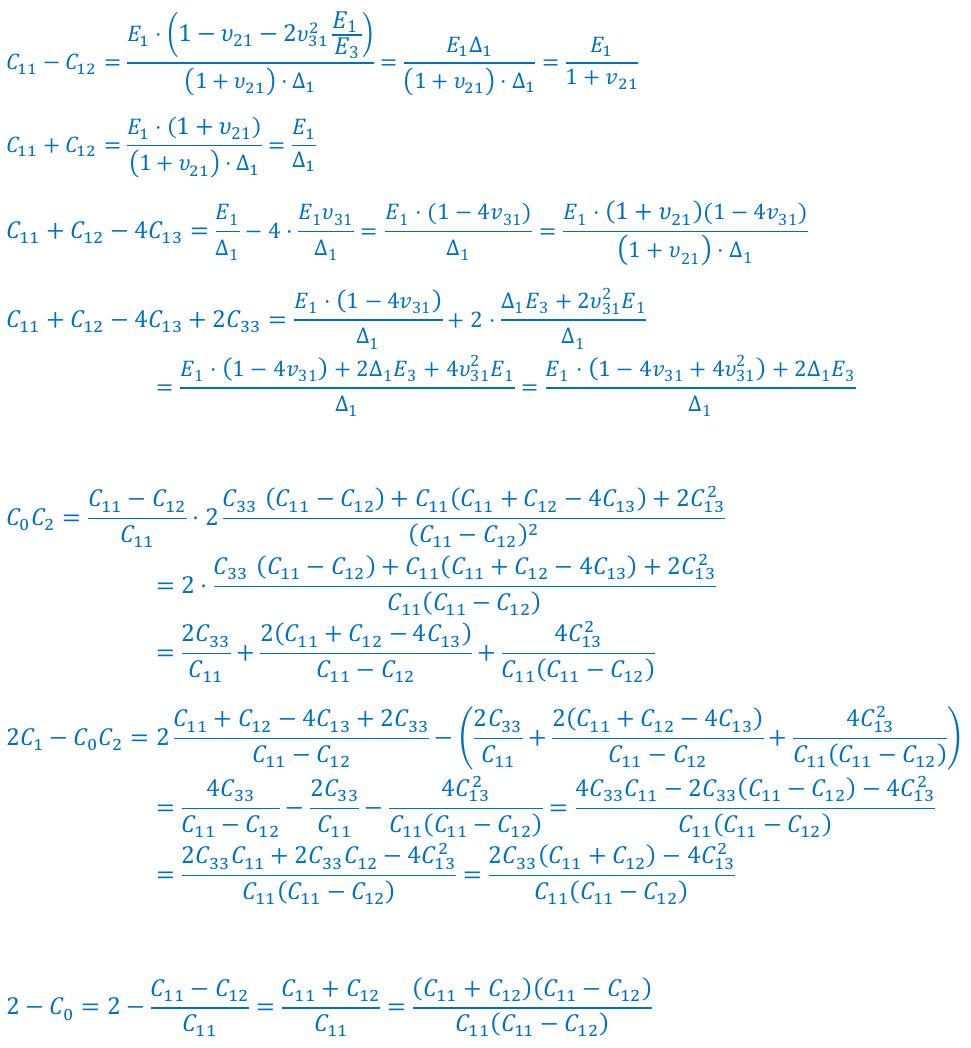
\includegraphics[max width=\textwidth]{2021_11_05---cohen-proof-of-lim-rahul-variable-manipulation}

Limit in Laplace Case
$$
\begin{gathered}
\lim _{t \rightarrow \infty} f(t)=\lim _{s \rightarrow 0} s \cdot F(s)=\frac{C_{1}-\frac{C_{2} \cdot C_{0}}{2}}{1-\frac{C_{0}}{2}} \cdot \lim _{s \rightarrow 0} s \cdot \tilde{\varepsilon}_{z z}=\frac{2 \cdot C_{1}-C_{2} \cdot C_{0}}{2-C_{0}} \cdot \lim _{s \rightarrow 0} s \cdot \tilde{\varepsilon}_{z z} \\
\lim _{s \rightarrow 0} s \cdot \tilde{\varepsilon}_{z z}=\dot{\varepsilon}_{0} \cdot t_{g} \cdot \lim _{s \rightarrow 0} \frac{1-\exp \left(-s \cdot t_{0} / t_{g}\right)}{s}=\dot{\varepsilon}_{0} t_{g} \cdot \lim _{s \rightarrow 0} \frac{\frac{t_{0}}{t_{g}} \exp \left(-s \cdot t_{0} / t_{g}\right)}{1}=\dot{\varepsilon}_{0} t_{g} \cdot \frac{t_{0}}{t_{g}}=\dot{\varepsilon}_{0} t_{0}
\end{gathered}
$$
$$
\begin{aligned}
\lim _{s \rightarrow 0} S \cdot F(s)=& \dot{\varepsilon}_{0} t_{0} \frac{2 \cdot C_{1}-C_{2} \cdot C_{0}}{2-C_{0}}=\dot{\varepsilon}_{0} t_{0} \frac{2 C_{33}\left(C_{11}+C_{12}\right)-4 C_{13}^{2}}{\left(C_{11}+C_{12}\right)\left(C_{11}-C_{12}\right)} \\
&=\dot{\varepsilon}_{0} t_{0} \frac{2 \frac{\Delta_{1} E_{3}+2 v_{31}^{2} E_{1}}{\Delta_{1}} \cdot \frac{E_{1}}{\Delta_{1}}-4\left(\frac{E_{1} v_{31}}{\Delta_{1}}\right)^{2}}{\frac{E_{1}}{\Delta_{1}} \cdot \frac{E_{1}}{1+v_{21}}\left(1+v_{21}\right)} \\
&=\dot{\varepsilon}_{0} t_{0}\left(1+v_{21}\right) \frac{2\left(\Delta_{1} E_{3}+2 v_{31}^{2} E_{1}\right) \cdot E_{1}-4 E_{1}^{2} v_{31}^{2}}{E_{1}^{2} \Delta_{1}} \\
&=2 \dot{\varepsilon}_{0} t_{0}\left(1+v_{21}\right)\left(\Delta_{1} \frac{E_{3}}{E_{1}}+2 v_{31}^{2}-2 v_{31}^{2}\right) \div \Delta_{1}=2 \dot{\varepsilon}_{0} t_{0}\left(1+v_{21}\right) \frac{E_{3}}{E_{1}} \\
&=\dot{\varepsilon}_{0} t_{0} \cdot 2\left(1+v_{21}\right) \frac{E_{3}}{E_{1}}=E_{3} \dot{\varepsilon}_{0} t_{0} \cdot \frac{2\left(1+v_{21}\right)}{E_{1}}
\end{aligned}
$$
Calculate the dimensional value as the solution provided was divided by (C11-C12)/2 to be nondimensional
$$
\begin{gathered}
\frac{C_{11}-C_{12}}{2}=\frac{E_{1}}{2\left(1+v_{21}\right)} \\
\lim _{s \rightarrow 0} s \cdot F(s) \cdot \frac{C_{11}-C_{12}}{2}=E_{3} \dot{\varepsilon}_{0} t_{0} \cdot \frac{2\left(1+v_{21}\right)}{E_{1}} \cdot \frac{E_{1}}{2\left(1+v_{21}\right)}=E_{3} \dot{\varepsilon}_{0} t_{0}
\end{gathered}
$$

\section{Summary}
$t \rightarrow \infty$ limit of Cohen's Laplace equation:
$$
\lim _{s \rightarrow 0} s \cdot F(s)=\dot{\varepsilon}_{0} t_{0} \cdot 2\left(1+v_{21}\right) \frac{E_{3}}{E_{1}}
$$
This can be dimensionalized to:
$$
\lim _{s \rightarrow 0} s \cdot F(s) \cdot \frac{C_{11}-C_{12}}{2}=E_{3} \dot{\varepsilon}_{0} t_{0}
$$
$$
\lim _{t \rightarrow \infty} f(t)=E_{3} \dot{\varepsilon}_{0} t_{0}
$$
Therefore the inversion equation and the Laplace equation are not exactly equal as specified only because they were divided by different values to become nondimensional. Thus, their dimensional values are the same.


\end{document}
